% experiment2.tex

\section{Experiment 2: Shallow Networks on MNIST}
\label{sec:experiment2}

TBD: This experiment trains two layer networks on MNIST using Abs and ReLU with and without the proposed initialization strategy. It also uses kMeans to train a nearest neighbor model to compare performance.

Experiment 2 explores the practicality of our distance metric interpretation of neural networks. Expanding from simpler models in Experiment 1, we train a two-layer feedforward network on the MNIST handwritten digit dataset. This experiment tests whether the Abs activation function and bias sampling improve performance in more complex, real-world tasks. We also interpret the linear nodes' representation using the L1 Mahalanobis distance framework.

Interpretation in Experiment 1 relied on the data representation ground truth. We no longer have that with MNIST. We introduce new techniques to distinguish between the Coherent and Adhoc representation classes that were identified in Experiment 1. We also find the mean input for each hidden node that represents a canonical reprsentation of the feature that node selects. We test whether an increase in Coherent nodes corresponds to improved model performance.


\subsection{Methodology}

We train a two-layer feedforward neural network on MNIST. Each layer is followed by either a ReLU or Abs activation function. The output layer also includes an activation function to ensure it functions as a distance metric, aligning with our presented theory. Weights are initialized He Normal Initialization. Bias initialization is tested between zeroing and data sampling, as introduced in Experiment 1.

We used cross entropy loss (CEL) as the model criterion. CEL expects the larger outputs to indicate class membership, but our distance metric framing treats smaller distances as indicating membership. To adapt our model to CEL, we negate the outputs of the final activation function.

We train ten models for each experimental condition.

The remaining model parameters are outlined in Table~\ref{tab:config_params_2}.

\begin{table}[h]
\centering
\caption{Configuration Parameters for Experiment 2}
\label{tab:config_params_2}
\begin{tabular}{ll}
\hline
Parameter & Value \\
\hline
Activation Functions & ReLU, Abs \\
Loss Function & CrossEntropyLoss \\
Optimizer & SGD \\
Epochs & 50 \\
Learning Rate & 0.001 \\
Momentum & 0.9 \\
Batch Size & 64 \\
Hidden Layer Size & 128 \\
Output Layer & Negated activation function \\
Weight Initialization & He Normal Initialization \\
Bias Initialization & Random or Sampled from Data \\
Dataset & MNIST (60,000 training samples, 10,000 test samples) \\
\hline
\end{tabular}
\end{table}

\subsection{Objectives and Hypotheses}

Building on our findings from Experiment 1, we hypothesize the following for Experiment 2:

\begin{itemize}
    \item \textbf{Abs vs. ReLU Hypothesis}: Abs and ReLU will perform similarly. Before the activation function is applied, the Abs node represents variance over \([- \delta .. + \delta]\), while the ReLU node represents variance over \([0 .. 2 \delta]\). Both should yield comparable overall performance despite these differences.
    
    \item \textbf{Bias Sampling Hypothesis}: Bias sampling continues to increase the number of Coherent features, even in more complex models like MNIST. This strategy should lead to better alignment of the network’s nodes with significant data clusters, improving both interpretability and model performance.
    
    \item \textbf{Coherent Features Hypothesis}: Models with a higher proportion of Coherent features will perform better than those with more Adhoc features. Coherent features align with meaningful clusters, leading to improved model generalization and accuracy.
    
    \item \textbf{Feature Interpretability Hypothesis}: Interpreting linear nodes as outputting distance metrics simplifies the understanding of the features that these nodes select, making the model’s internal structure easier to interpret.
\end{itemize}

\subsection{Results and Discussion}

\subsubsection{Performance Results}

Table~\ref{tab:ex2_results_table} summarizes the performance metrics across the different experimental conditions. We report the average accuracy, precision, recall, F1 score, and test error, along with the minimum and maximum accuracy to give a sense of variability across the ten models trained for each condition. We also include metrics for model diversity to measure the number of differing predictions between models within the same condition.

\begin{table}[h]
    \centering
    \caption{Performance Results for Experimental Conditions}
    \label{tab:ex2_results_table}
    \begin{tabular}{l|c|c|c|c}
    \hline
    Metric & ReLU & ReLU + Bias Sampling & Abs & Abs + Bias Sampling \\
    \hline
    Accuracy (Avg) & 0.9773 & 0.9770 & 0.9749 & 0.9773 \\
    Accuracy (Min) & 0.9759 & 0.9756 & 0.9554 & 0.9728 \\
    Accuracy (Max) & 0.9785 & 0.9779 & 0.9799 & 0.9795 \\
    Precision & 0.9772 & 0.9769 & 0.9750 & 0.9772 \\
    Recall & 0.9771 & 0.9768 & 0.9747 & 0.9771 \\
    F1 Score & 0.9771 & 0.9768 & 0.9748 & 0.9771 \\
    Test Error & 0.0747 & 0.0757 & 0.0855 & 0.0754 \\
    Avg Error Count & 227.0 & 230.3 & 250.9 & 227.1 \\
    Unique Errors & 509 & 509 & 805 & 617 \\
    Consistent Errors & 70 & 79 & 47 & 40 \\
    Voting Errors & 213 & 215 & 205 & 204 \\
    L2 Errors & 188 & 185 & 163 & 163 \\
    \hline
    \end{tabular}
    \end{table}
    
Figure~\ref{fig:ex2_training_test_error} presents two graphs: one showing the average training error and another showing the average test error for each configuration, displayed side by side. These curves provide insight into the learning dynamics and generalization performance of the models.


\begin{figure}[h]
    \centering
    % Placeholder for training and test error plots
    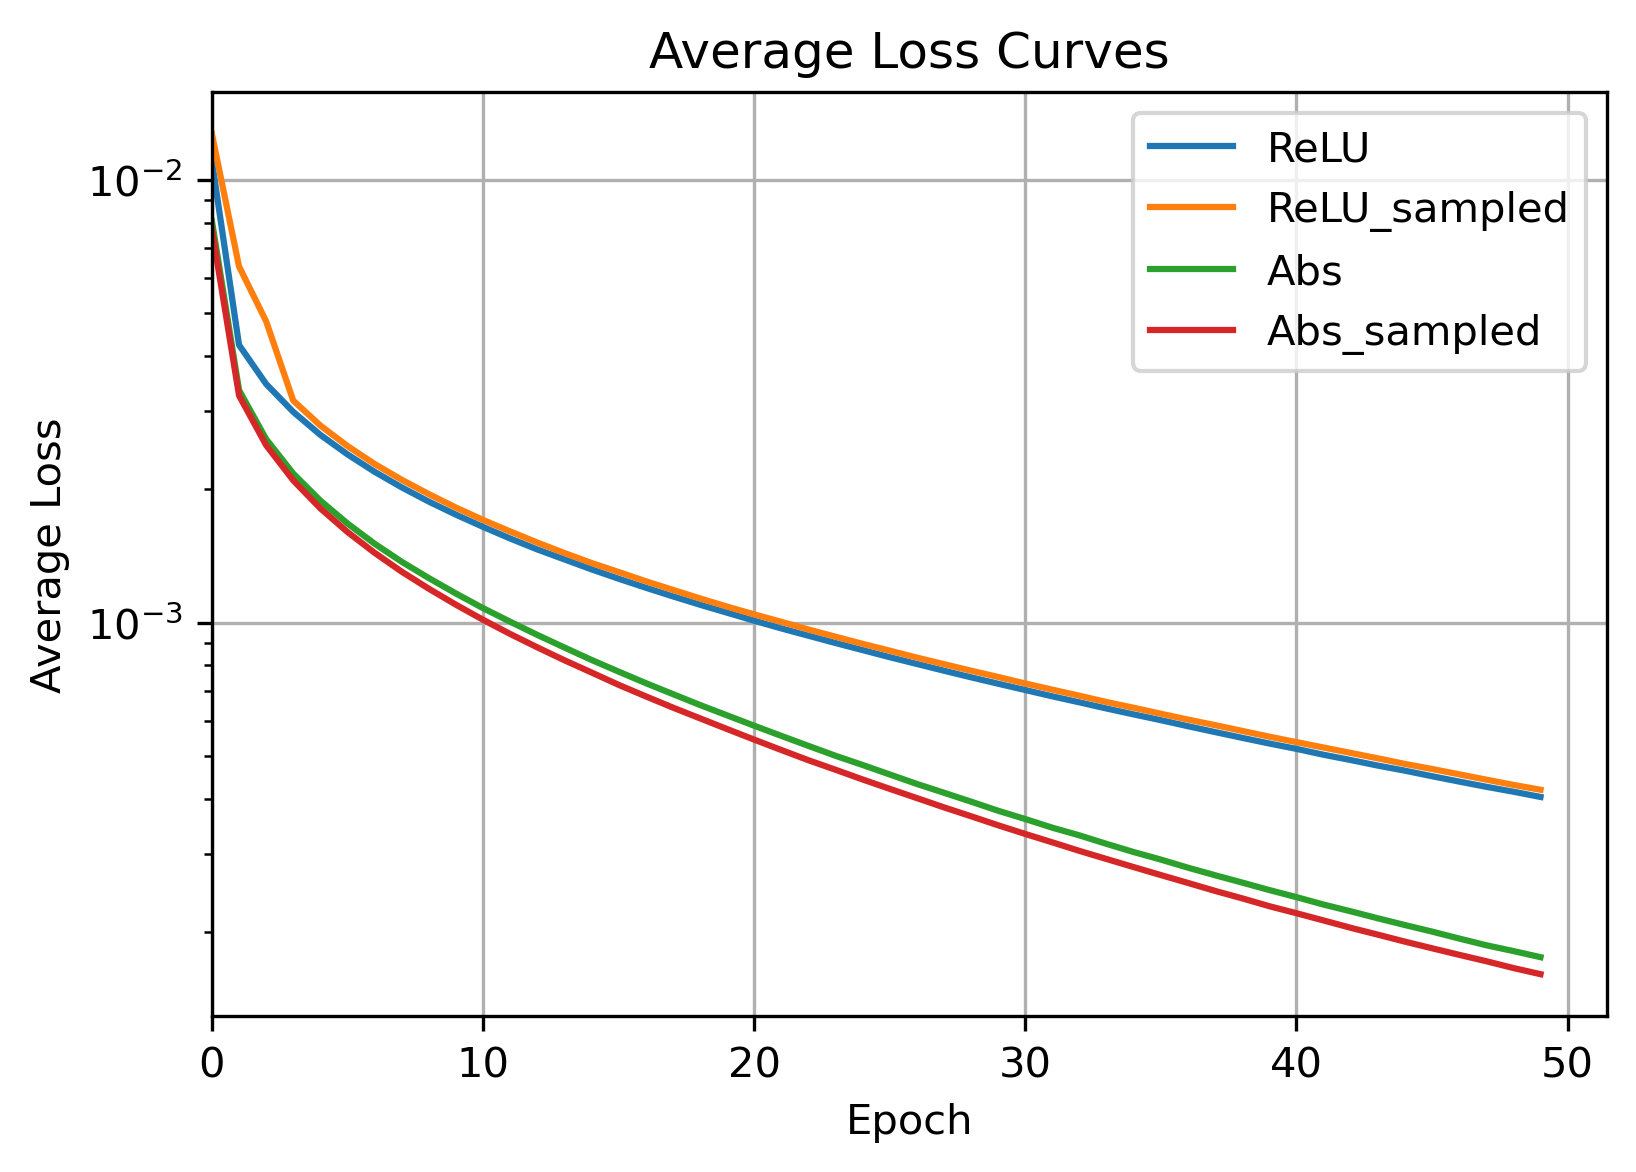
\includegraphics[width=0.45\textwidth]{ex2_training_error.png}
    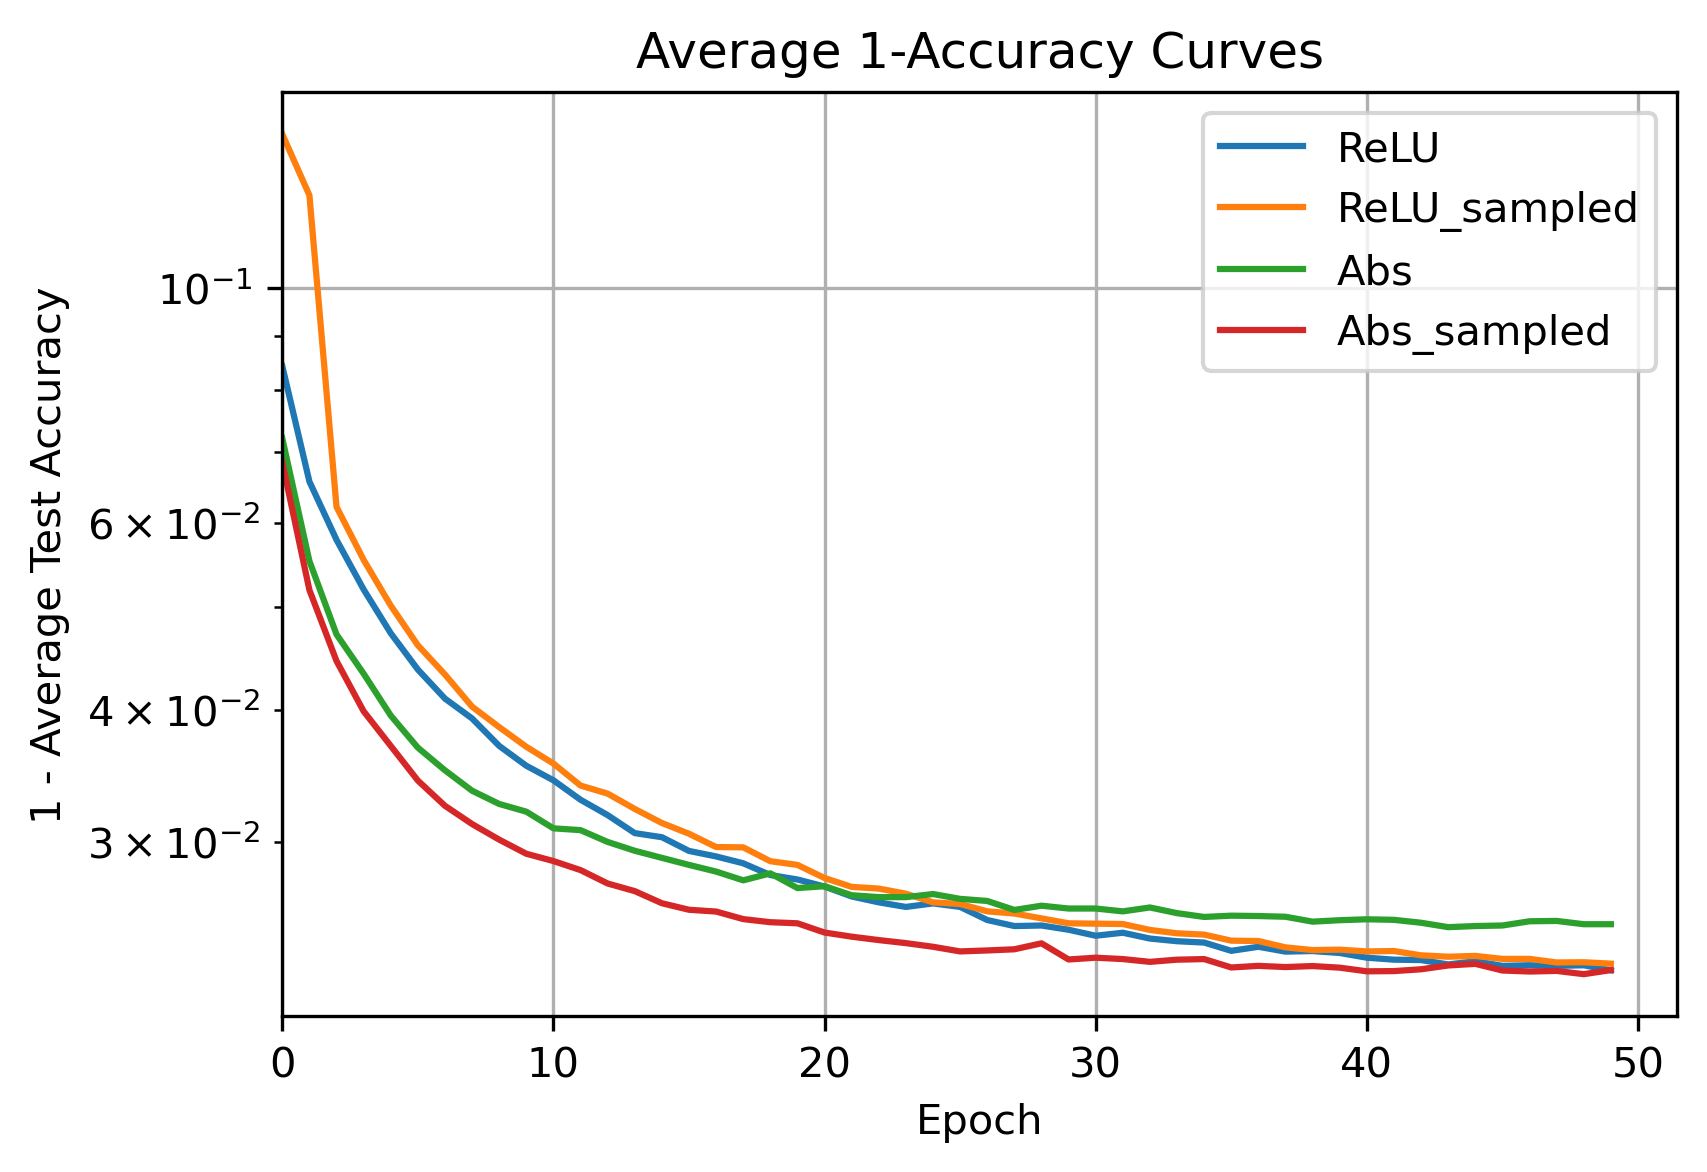
\includegraphics[width=0.45\textwidth]{ex2_test_accuracy.png}
    \caption{Training and test error curves for each experimental condition. The left plot shows the average training error, while the right plot shows the average test error. Both curves are averaged over the ten models trained for each condition.}
    \label{fig:ex2_training_test_error}
\end{figure}


\subsection{Results and Discussion}
\label{sec:results_discussion}

The performance metrics summarized in Table~\ref{tab:ex2_results_table} and Figure~\ref{fig:ex2_training_test_error} provide comprehensive insights into the effectiveness and diversity of the trained models under different experimental conditions. Each metric is averaged over ten trained models per configuration, ensuring robust statistical significance.

\paragraph{Accuracy and Performance Metrics}

All experimental configurations achieved high average accuracy on the MNIST dataset, ranging from \textbf{97.0\%} to \textbf{97.73\%}, indicating strong overall performance. Specifically, both ReLU and Abs activation functions with bias sampling attained an average accuracy of \textbf{97.73\%}. In contrast, Abs-activated models without bias sampling achieved a slightly lower average accuracy of \textbf{97.49\%}, accompanied by a broader accuracy range from \textbf{95.54\%} to \textbf{97.99\%}. This wider range for Abs without bias sampling suggests greater variability in feature learning across different training runs, potentially indicating underfitting. The higher variability is further supported by the increased number of unique errors (805) in Abs models without bias sampling compared to ReLU models (509), highlighting diverse feature representations that may not consistently capture the underlying data structure.

Precision, Recall, and F1 Score metrics are closely aligned with the observed accuracy trends. Abs-activated models without bias sampling demonstrate slightly lower Precision (\textbf{97.50\%}), Recall (\textbf{97.47\%}), and F1 Score (\textbf{97.48\%}) compared to ReLU configurations (\textbf{Precision}: 97.72\%, \textbf{Recall}: 97.71\%, \textbf{F1 Score}: 97.71\%). This minor discrepancy aligns with the broader accuracy range and higher unique error counts, indicating that while Abs models are effective, their varied feature learning may introduce inconsistencies in classification.

\paragraph{Model Diversity Metrics}

The model diversity metrics offer valuable perspectives on the consensus and variability among the trained models. Abs models without bias sampling exhibit a significantly higher number of unique errors (805), indicating that a larger number of test data points were misclassified by at least one model. In comparison, ReLU models recorded 509 unique errors, and Abs models with bias sampling had 617 unique errors. This high unique error count in Abs models without bias sampling suggests that these models are learning a more diverse set of features, capturing varied aspects of the data but at the cost of consistency across different training runs.

Consistent errors, defined as data points misclassified by all models within a configuration, remain relatively low across all conditions. Abs models with bias sampling recorded the fewest consistent errors (40), whereas ReLU models without bias sampling had the highest count (79). This indicates that bias sampling effectively reduces systematic misclassifications, promoting greater alignment with significant data clusters and enhancing overall model reliability.

Voting Errors, representing the number of data points misclassified by five or more models, are comparable across all configurations, ranging from 204 to 215. This similarity suggests that ensemble methods would encounter similar levels of misclassification regardless of activation function or initialization strategy \cite{dietterich2000ensemble}. Additionally, L2 Errors, which assess the distance metric predictions by computing the L2 norm of the prediction vectors, remain consistent across all experimental conditions (163-188), indicating stable distance-based representations.

\paragraph{Implications for Hypotheses}

The experimental results align with the proposed hypotheses in several ways:

\begin{itemize}
    \item \textbf{Abs vs. ReLU Performance}: Abs and ReLU activations exhibit similar average accuracies when bias sampling is employed. However, Abs activations without bias sampling show greater variability and higher unique error counts, supporting the hypothesis that Abs can capture diverse features but may require effective initialization to maintain consistency.
    
    \item \textbf{Bias Sampling Effectiveness}: The bias sampling initialization strategy consistently enhances model performance and reduces unique errors, particularly for Abs activations. This supports the hypothesis that bias sampling promotes better alignment with significant data clusters, thereby improving both interpretability and model performance.
    
    \item \textbf{Model Diversity and Underfitting}: The increased accuracy range and unique errors in Abs models without bias sampling suggest potential underfitting, as these models may benefit from additional hidden nodes to represent a more comprehensive set of features. This observation aligns with the hypothesis that higher model diversity can capture varied data aspects but may introduce inconsistencies.
\end{itemize}

Overall, Experiment 2 demonstrates that while both Abs and ReLU activation functions are effective in training shallow networks on the MNIST dataset, the combination of Abs activations with bias sampling initialization offers enhanced performance consistency and interpretability. The observed model diversity metrics highlight the trade-offs between feature richness and classification consistency, guiding future architectural and initialization strategies for optimizing neural network performance.


% Present the results comparing Abs and ReLU activations, as well as comparisons with K-means and Gaussian nearest neighbor implementations.

